\documentclass[a4paper]{article}

\def\ncourse {Theoretical Astroparticle Physics}
\def\ntopic {The Early Universe}
 
\makeatletter

%Title
\def\nauthor{Matteo Zandi}

\title{\huge \ncourse \\ \Large \ntopic}

\author{\color{mycolor}\nauthor}
\date{\today}

%Size
\usepackage{geometry}
%\geometry{a4paper, top = 4cm, bottom = 4cm, left = 3cm, right = 4cm}
\geometry{
    papersize={379pt, 699pt},
    textwidth=345pt,
    textheight=596pt,
    left=17pt,
    top=54pt,
    right=17pt
  }

%Package
\usepackage{lipsum}
\usepackage{xcolor} \xdefinecolor{mycolor}{RGB}{0,175,179} 
\usepackage{hyperref} \hypersetup{colorlinks, linkcolor={mycolor}, citecolor={mycolor}, urlcolor={mycolor}}
\usepackage{titlesec}
\titleformat{\section}{\newpage\normalfont\Large\bfseries\color{mycolor}\centering}{\thesection}{1em}{}
\titleformat{\subsection}{\normalfont\large\bfseries\color{mycolor}\centering}{\thesubsection}{1em}{}
\titleformat{\subsubsection}{\normalfont\bfseries\color{mycolor}\centering}{\thesubsubsection}{1em}{}

%Commands

\usepackage[backend=bibtex, sorting=none]{biblatex}
\addbibresource{../bibliography.bib}


\usepackage{amsmath}
\usepackage{amsthm}
\usepackage{thmtools}
\usepackage{mathtools}
\usepackage{amsfonts}
\usepackage{dsfont}
\usepackage{yfonts}
\usepackage{amssymb}
\usepackage{cancel}
\usepackage{slashed}
\usepackage{feynmp-auto}


\newtheorem{principle}{Principle}[section]
\newtheorem{lemma}{Lemma}[section]
\theoremstyle{definition}
\newtheorem{example}{Example}[section]
\newtheorem{exercise}{Exercise}[section]
\renewcommand\qedsymbol{q.e.d.}

\let\oldproof\proof
\renewcommand{\proof}{\color{darkgray}\oldproof}

\theoremstyle{remark}
\newtheorem{case}{Case}

\newtheoremstyle{colored}{}{}{\itshape}{}{\color{mycolor}\normalfont\bfseries\indent}{}{\newline}{}

\declaretheorem[
  style=colored,
  name=Definition,
  numberwithin=section,
]{definition}

\declaretheorem[
  style=colored,
  name=Theorem,
  numberwithin=section,
]{theorem}

\declaretheorem[
  style=colored,
  name=Corollary,
  numberwithin=section,
]{corollary}

\declaretheorem[
  style=colored,
  name=Law,
  numberwithin=section,
]{law}

\declaretheorem[
  style=colored,
  name=Principle,
  numberwithin=section,
]{princ}

\newcommand{\dv}[2]{\frac{d#1}{d#2}}
\newcommand{\dvin}[3]{\frac{d#1}{d#2}\Big\vert_{#3}}
\newcommand{\dvd}[2]{\frac{d^2#1}{d#2^2}}
\newcommand{\dvf}[2]{\frac{\delta #1}{\delta #2}}
\newcommand{\pdv}[2]{\frac{\partial#1}{\partial#2}}
\newcommand{\pdvd}[3]{\frac{\partial^2 #1}{\partial#2 \partial#3}}
\newcommand{\pdvdu}[2]{\frac{\partial^2 #1}{\partial#2^2}}
\newcommand{\integ}[3]{\int_{#1}^{#2}d#3~}
\newcommand{\poi}[2]{[#1,~#2]}
\newcommand{\poiexp}[2]{\pdv{#1}{q^i} \pdv{#2}{p_i} - \pdv{#2}{q^i} \pdv{#1}{p_i}}

\newcommand{\comm}[2]{[#1,~#2]}
\newcommand{\set}[2]{\{#1\colon#2\}}
\newcommand{\inner}[2]{\langle#1,~#2\rangle}
\newcommand{\av}[1]{\langle#1\rangle}
\newcommand{\avp}[2]{\langle#1\rangle_{#2}}
\newcommand{\ket}[1]{\vert#1\rangle}
\newcommand{\bra}[1]{\langle#1\vert}
\newcommand{\braket}[2]{\langle#1\vert#2\rangle}  
  
\begin{document} 
 
\maketitle 

\begin{abstract}
    In this notes, we wiil study thermodynamics of the early universe from a particle physics point of view.
\end{abstract}


\tableofcontents
\newpage

\section{Cosmology}

    In this chapter, we will study the cosmology.

\subsection{Hubble's law}

    The Universe is expanding according to the Hubble's law
    \begin{equation}\label{hubble}
        v = H_0 d ~,
    \end{equation}
    where $v$ is the radial velocity, $d$ is the distance and $H_0$ is the Hubble constant, whose current value is estimated to be
    \begin{equation*}
        H_0 \sim 70 ~ km ~ s^{-1} ~ Mpc ~, \quad H_0 \sim h 100 ~ km ~ s^{-1} ~ Mpc ~,
    \end{equation*}
    where $h$ is the Hubble parameter. Consider two points in the spacetime. Their comoving distance $x$ attached spacetime is independent on time but their physical distance $d$ is related to time by 
    \begin{equation}\label{distance}
        d = a(t) x ~,
    \end{equation}
    where $a(t)$ is the scale factor. 
    Combining together~\eqref{hubble} and~\eqref{distance}, we can find the relation between Hubble constant and the scale factor
    \begin{equation*}
        v = \dot d = \dot a (t) x = H(t) d(t) = H(t) a(t) x ~, \quad H(t) = \frac{\dot a(t)}{a(t)} ~.
    \end{equation*}

\subsection{Friedmann-Robertson-Walker metric}

    Our assumptions about the Universe is the cosmological principle, which states that the Universe is homogeneous and isotropic at large scales. This The metric associated to this spacetime is the so-called Friedmann-Robertson-Walker metric
    \begin{equation*}
        ds^2 = dt^2 - a^2 (t) \Big ( \frac{dr^2}{1 - k r^2} + r^2 d\Omega^2 \Big ) ~,
    \end{equation*}
    where $k$ is a parameter that tells us what is the geometry of spacetime: 
    \begin{enumerate}
        \item for $k = 0$, the spacetime is flat (parallel lines stay at the same distance);
        \item for $k = 1$, the spacetime is closed (parallel lines always intersect)
        \item for $k = -1$, the spacetime is open (parallel lines get further away from each others).
    \end{enumerate}
    For a Universe with free non-interacting particles $P^\mu_i$ moving along $r_i(t)$, the energy-momentum tensor is to be
    \begin{equation*}
        T^{\mu 0} = \sum_i p_i^\mu t \delta ( r - r_i(t)) , \quad T^{\mu j} = \sum_i p_i^\mu t \dv{x^i}{t} \delta ( r - r_i(t)) ~,
    \end{equation*}
    or, using density and pressure, 
    \begin{equation*}
        T^{00} = c^2 \rho ~, \quad T^{0i} = 0 ~, \quad T^{ij} = p \delta^{ij} ~.
    \end{equation*}
    Therefore, Einstein's equation (with the continuity equation)
    \begin{equation*}
        G_{\mu\nu} (a(t), k) \propto T_{\mu\nu} (\rho, p, \Lambda) ~, \quad \partial_\mu T^{\mu\nu} = 0 ~,
    \end{equation*} 
    becomes the so-called Friedmann's equation
    \begin{equation*}
        \Big ( \frac{\dot a}{a} \Big)^2 + \frac{k}{a^2} = \frac{8 \pi G_N}{3} \rho + \frac{\Lambda}{3} , \quad \frac{\ddot a}{a} = - \frac{4 \pi G_N}{3} (\rho + 3 p) + \frac{\Lambda}{3} ~.
    \end{equation*}
    Our unknowns are $a$ and $k$. About $a$, we can distinuish three possible cases:
    \begin{enumerate}
        \item for a matter dominated Universe, i.e.~$p = 0$ and $\Lambda = 0$, the solution of these equations is 
        \begin{equation*}
            \rho_m \propto a^{-3} ~, \quad  a(t) \propto t^{2 / 3} ~;
        \end{equation*}
        \item for a radiation dominated Universe, i.e.~$p = \rho / 3$ and $\Lambda = 0$, the solution of these equations is 
        \begin{equation*}
            \rho_r \propto a^{-4} ~, \quad  a(t) \propto t^{1 / 2} ~;
        \end{equation*}
        \item for a $\Lambda$ dominated Universe, i.e.~$p = - \rho$ and $\Lambda \neq 0$, the solution of these equations is 
        \begin{equation*}
            \rho_m \propto const ~, \quad  a(t) \propto e^{\sqrt{\frac{\Lambda}{3}} t} = e^{H t} ~.
        \end{equation*}
    \end{enumerate}
    About $k$, in order to understand what is the curvature of the Universe, we can express it in terms of the density parameter 
    \begin{equation*}
        \Omega = \frac{\rho}{\rho_{crit}} ~, \quad \rho_{crit} = \frac{3 H^2}{8 \pi G_N} ~,
    \end{equation*}
    \begin{equation*}
        \frac{k}{a^2} = \frac{8 \pi G_N}{3} \rho - H^2 ~,
    \end{equation*}
    so that, if $rho = \rho_{crit}$ or $\Omega = 1$, we have a flat Universe $K=0$. Experimental data support a flat expanding Universe. independent
    \begin{equation*}
        H^2(z) = H_0^2 ( \Omega_{\Lambda} + \Omega_{b} (1 + z)^2 + \Omega_{dm} (1 + z)^3 + \Omega_{\gamma} (1 + z)^4 ) ~,
    \end{equation*}
    \begin{equation*}
        H^2(a) = H_0^2 ( \Omega_{0\Lambda} + \Omega_{0k} a^{-2} + \Omega_{0m} a^{-3} + \Omega_{0\gamma} a^{-4} ) ~,
    \end{equation*}
    where
    \begin{enumerate}
        \item $\Omega_{0\Lambda} = 0.679 \pm 0.013$;
        \item $\Omega_{0b} h^2 = 0.0224 \pm 0.0001$;
        \item $\Omega_{0m} = 0.315 \pm 0.007$;
        \item $\Omega_{0\gamma} \sim 0$;
        \item $\Omega_{0k} = 0.001 \pm 0.002$.
    \end{enumerate}

    
\section{Thermodynamics of the early Universe}

    Since the Universe is isotropic, the equilibrium phase space distribution function depends only on the modulus of the momentum $|\mathbf p|$ and it will be Fermi-Dirac for fermions and Bose-Einstein for bosons
    \begin{equation*}
        f(p) = (e^{\frac{E - \mu}{T}} \pm 1)^{-1} ~,
    \end{equation*}
    where $E = \sqrt{p^2 + m^2}$, $\mu$ is the chemical potential, which can be neglected due to asymmetry between particles and antiparticles. With this function, we can calculate thermodynamic quantities, like number density
    \begin{equation*}
        n = \frac{g}{(2\pi)^3} \int d^3 p f(t, p) ~,
    \end{equation*}
    energy density
    \begin{equation*}
        \rho = \frac{g}{(2\pi)^3} \int d^3 f(t, p) E(t, p)
    \end{equation*}
    or pressure
    \begin{equation*}
        p = \frac{g}{(2\pi)^3} \int d^3 p f(t, p) \frac{|\mathbf p|^2}{3 E} ~.
    \end{equation*}
    The number of degrees of freedom $g$ is 
    \begin{enumerate}
        \item $g = 1$ for real scalars;
        \item $g=2$ for massless vector bosons, complex scalars or Maiorana fermions, 
        \item $g = 3$ for massive vector bosons;
        \item $g = 4$ for Dirac fermions.
    \end{enumerate}

    In the particular case of relativistic species, i.e. $T \gg m$ and $\mu = 0$, we have 
    \begin{equation*}
        n_{bos} \simeq g \frac{T^3}{\pi^2} \zeta (3) ~, \quad n_{fer} \simeq \frac{3}{4} n_{bos} ~,
    \end{equation*}
    \begin{equation*}
        \rho_{bos} \simeq \frac{\pi^2}{30} g T^4 ~, \quad \rho_{fer} \simeq \frac{7}{8} \rho_{bos} ~, \quad p = \frac{\rho}{3} ~.
    \end{equation*}
    Notice that the number density goes as $n \sim T^3$, whereas energy density goes as $\rho \sim T^4$.

    In the particular case of non-relativistic species, i.e. $T \ll m$, we have 
    \begin{equation*}
        n = g \Big ( \frac{m T}{2 \pi} \Big )^{3/2} e^{- \frac{m - \mu}{T}} ~, \quad \rho = m n ~.
    \end{equation*}
    Notice that in the number density, there is an exponential suppression.

    The entropy density is 
    \begin{equation*}
        s = \frac{2 \pi^2}{45} g_{*s} T_\gamma^3 ~,
    \end{equation*}
    where the number of relativistic degrees of freedom is given by
    \begin{equation*}
        g_{*s} = \sum_{relativistic bosons} g_i \Big ( \frac{T_i}{T_\gamma} \Big )^3 + \frac{7}{8} \sum_{relativistic fermions} g_i \Big ( \frac{T_i}{T_\gamma} \Big )^3 ~.
    \end{equation*}
    Entropy is conserved, since the Universe is all there is, so that 
    \begin{equation*}
        d (s a^3) = 0 ~, \quad T_\gamma \sim g_{*3}^{-1/3} a^{-1} ~.
    \end{equation*}
    Every time a relativistic particle becomes non-relativistic, due to the expansion of the Universe, entropy is transfered into an increase of the temperature of the plasma (even though it contributes as a small perturbation compared to the expansion of the universe temperature). Regarding energy density 
    \begin{equation*}
        \rho_{rel} = \frac{\pi}{30} g_* T^4  ~,
    \end{equation*}
    where the number of relativistic degrees of freedom is given by
    \begin{equation*}
        g_{*} = \sum_{relativistic bosons} g_i \Big ( \frac{T_i}{T_\gamma} \Big )^4 + \frac{7}{8} \sum_{relativistic fermions} g_i \Big ( \frac{T_i}{T_\gamma} \Big )^4 ~.
    \end{equation*}

    \begin{figure}
    \centering
    \begin{tabular}{ c | c | c | c | c || c} 
        particle & flavors & colors & spins & antiparticle & total \\ 
        \hline
        gluons & - & 8 & 2 & -  & 16 \\ 
        photon & - & - & 2 & - & 2 \\ 
        massive vector bosons & 3 & - & 3 & - & 9 \\ 
        Higgs boson & - & - & - & - & 1 \\ 
        \hline
        \hline
        & & & & & 28 \\
    \end{tabular} 
    \caption{Number of degrees of freedom for the bosons in the Standard Model.}
    \end{figure}

    \begin{figure}
    \centering
    \begin{tabular}{ c | c | c | c | c || c } 
        particle & flavors & colors & spins & antiparticle & total \\ 
        \hline
        quarks & 6 & 3 & 2 & 2  & 72 \\ 
        leptons & 3 & - & 2 & 2 & 12 \\ 
        neutrinos & 3 & - & - & 2 & 6 \\ 
        \hline
        \hline
        & & & & & 90 \\
    \end{tabular} 
    \caption{Number of degrees of freedom for the fermions in the Standard Model.}
    \end{figure}

    An estimate to $g_* = g_{*s}$ for a single plasma in in Figure \ref{dof}. 
    \begin{figure}[ht!]
        \centering
        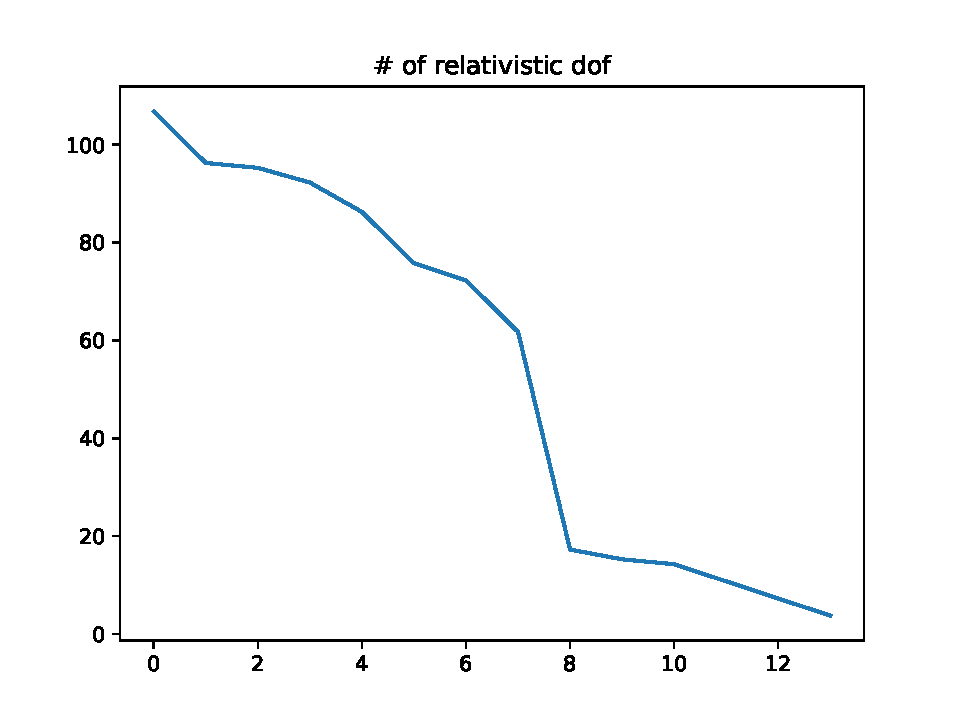
\includegraphics[width=10cm]{dof.pdf}
        \caption{Number of relativistic degrees of freedom as a function of time.}
        \label{dof}
    \end{figure}


\nocite{taplecture} 
\nocite{kolbturner}  
\printbibliography

\immediate\write18{mv \jobname.pdf ../../../pdf/\jobname.pdf}
\end{document}

